\documentclass[12pt,openright,twoside,a4paper,english,french,spanish]{abntex2}

\usepackage{cmap}	
\usepackage{lmodern}	
\usepackage[T1]{fontenc}	
\usepackage[utf8]{inputenc}
\usepackage{lastpage}		
\usepackage{indentfirst}
\usepackage{color}	
\usepackage{graphicx}	
\usepackage{units}
\usepackage[brazilian,hyperpageref]{backref}
\usepackage[alf]{abntex2cite}
\usepackage{bold-extra}
\usepackage{eso-pic}
\usepackage{siunitx}
\usepackage{listings}
\usepackage{caption}
\usepackage{hyperref}
\usepackage{adjustbox}
\usepackage{booktabs}
\renewcommand{\backrefpagesname}{Citado na(s) página(s):~}
\renewcommand{\backref}{}
\renewcommand*{\backrefalt}[4]{
	\ifcase #1 %
		Nenhuma citação no texto.%
	\or
		Citado na página #2.%
	\else
		Citado #1 vezes nas páginas #2.%
	\fi}%
% ---


\newcommand{\curso}[1]{\def\imprimircurso{#1}}

\newcommand{\palavraChaveUm}[1]{\def\imprimirpalavrachaveum{#1}}
\newcommand{\palavraChaveDois}[1]{\def\imprimirpalavrachavedois{#1}}

\newcommand{\cdu}[1]{\def\nomecdu{#1}}
\newcommand{\dataDaAprovacao}[1]{\def\imprimirdatadaaprovacao{#1}}

\newcommand{\membroConvidadoUm}[1]{\def\imprimirmembroconvidadoum{#1}}
\newcommand{\membroConvidadoDois}[1]{\def\imprimirmembroconvidadodois{#1}}

\newcommand\BackgroundPic{%
	\put(0,0){%
		\parbox[b][\paperheight]{\paperwidth}{%
			\vfill
			\centering
			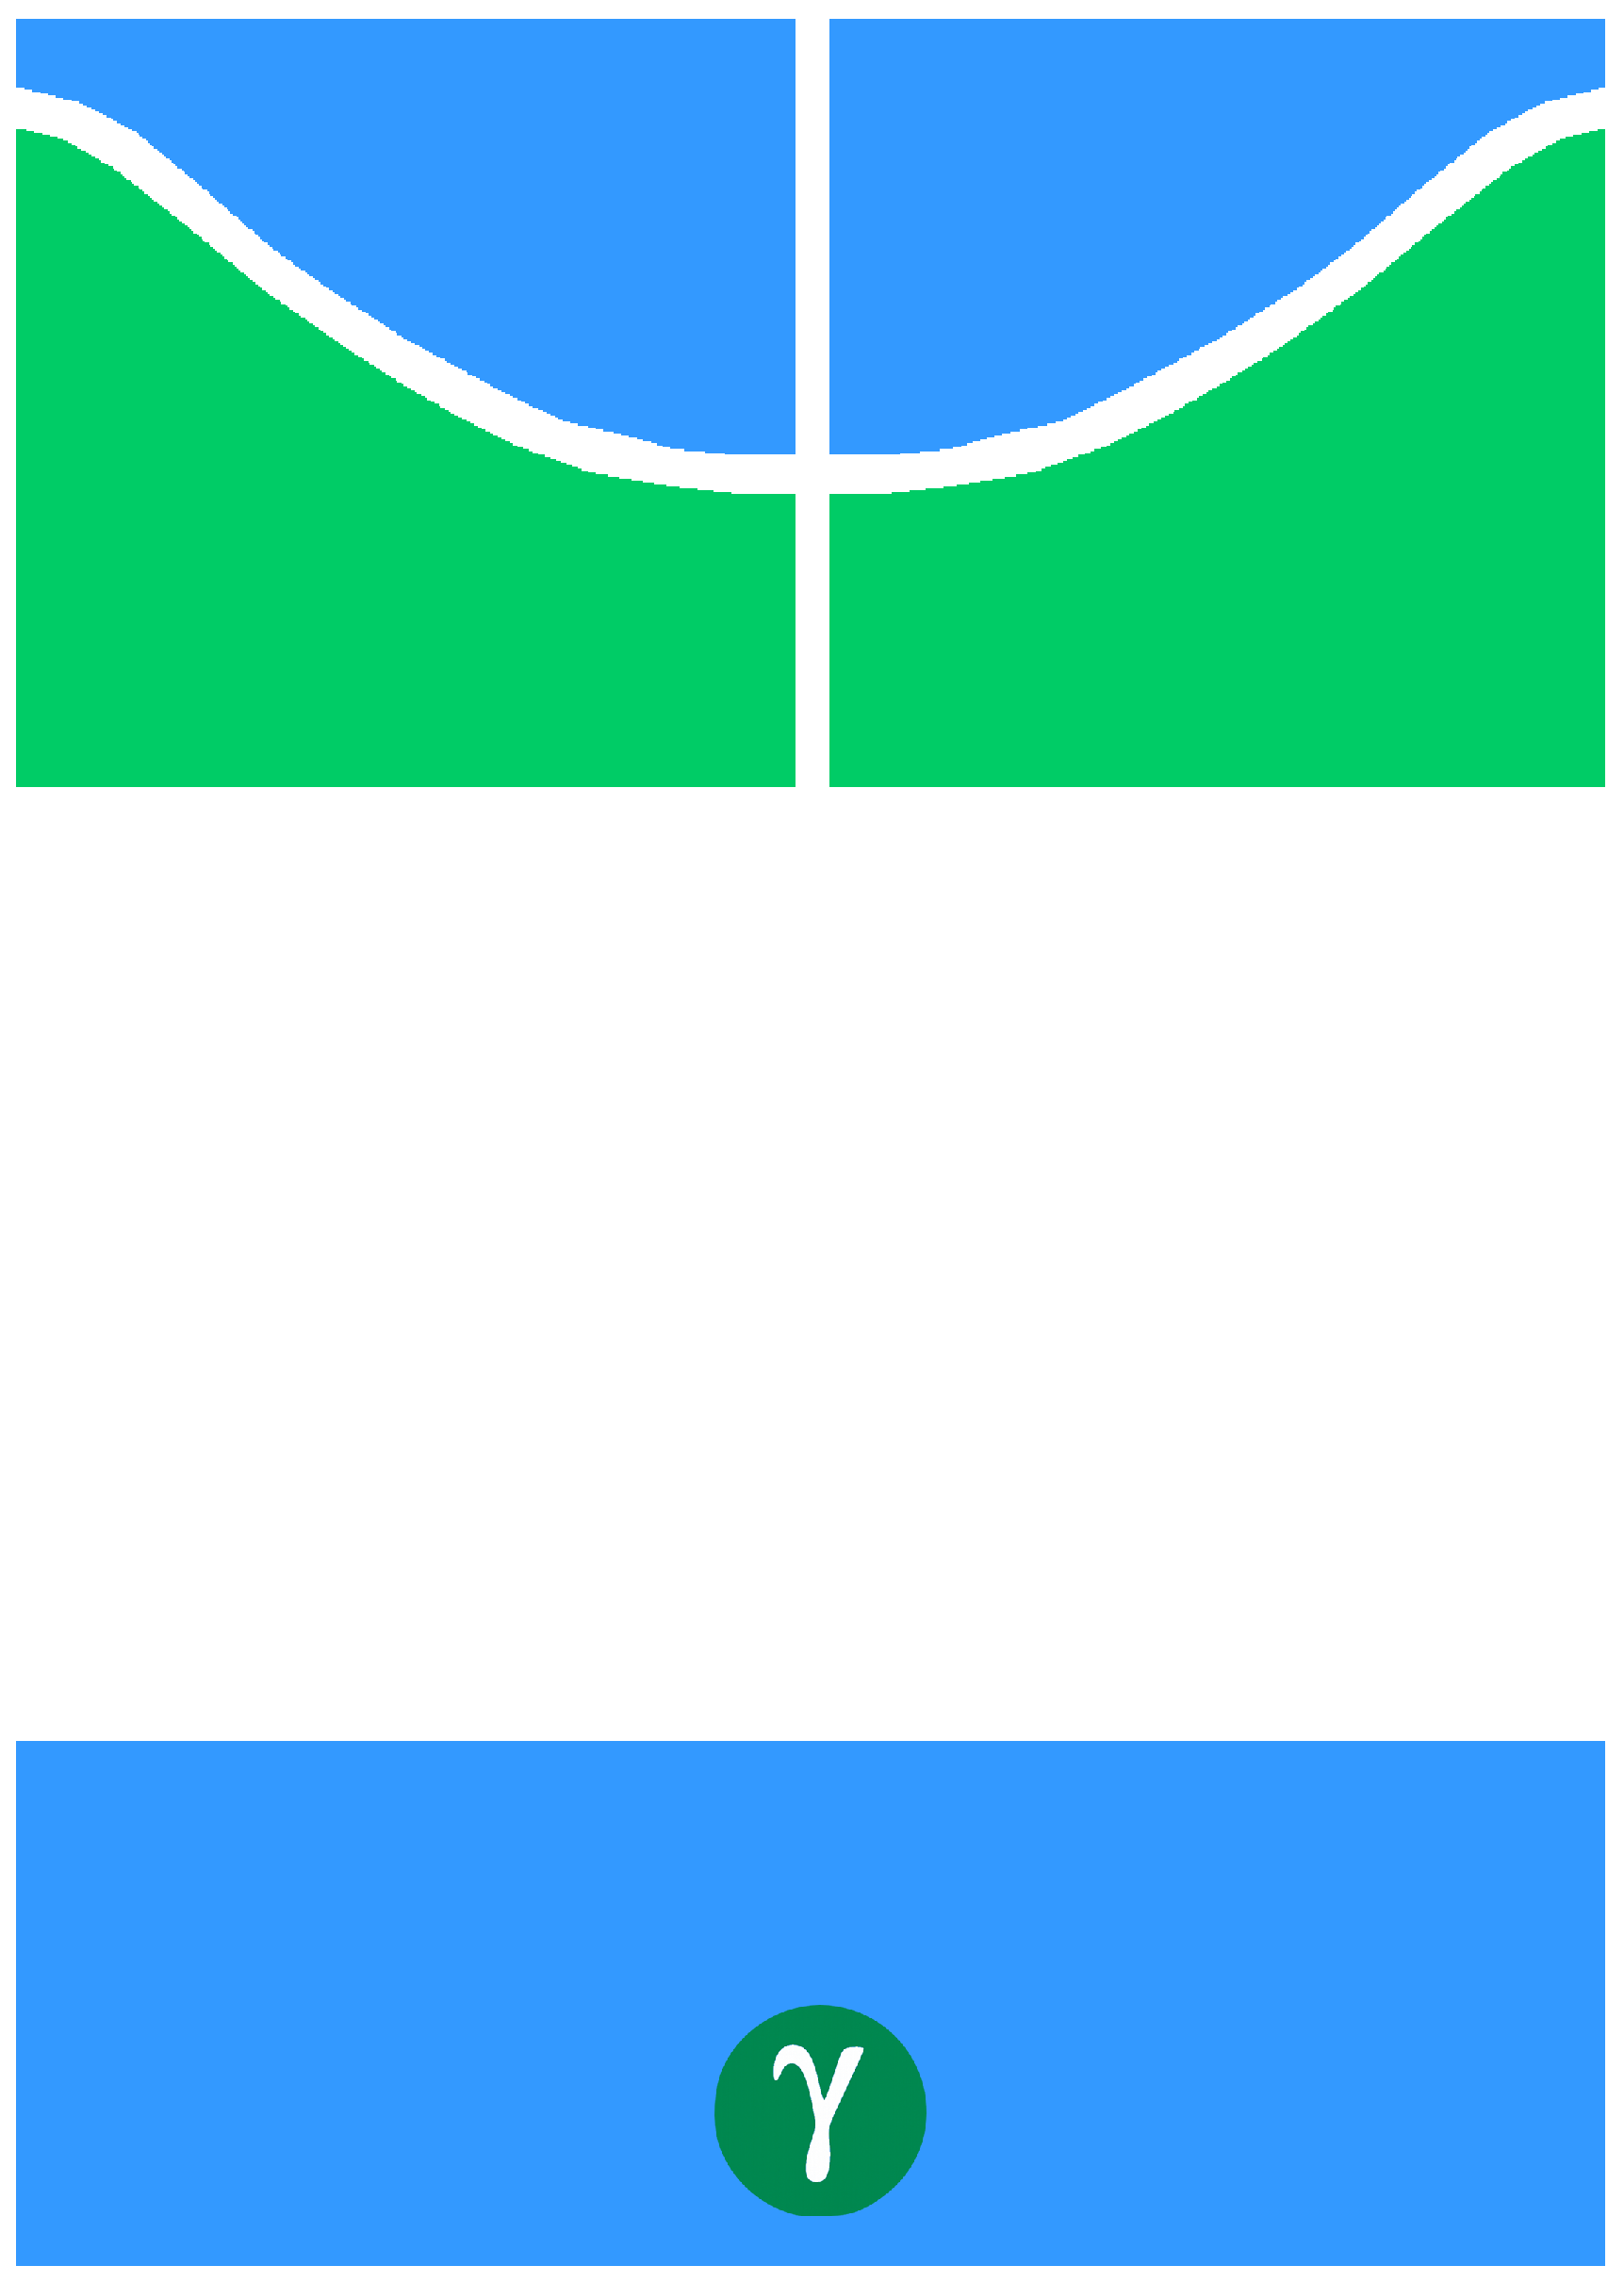
\includegraphics[width=\paperwidth,height=\paperheight,%
				keepaspectratio]{figuras/capa.eps}%
			\vfill
		}
	}
}

\renewcommand{\imprimircapa}{%
  \begin{capa}%
    \center
	\AddToShipoutPicture*{\BackgroundPic}

    \vspace*{2.7in}
	{\textbf{\large\imprimirinstituicao}}
	\par
	{\textbf{\large\imprimircurso}}

	\vspace{0.5in}

    {\ABNTEXchapterfont\bfseries\LARGE\imprimirtitulo}
    \vspace*{\fill}
    
	\begin{flushright}
    	\textbf{{\large{Autores: \imprimirautor}}}
		\par
    	\textbf{{\large{Orientador: \imprimirorientador}}}
    	\par
    	\textbf{{\large{Coorientador: \imprimircoorientador}}}
	\end{flushright}
		
    \vspace*{0.2in}
    \textbf{{\large\imprimirlocal}}
    \par
    \textbf{{\large\imprimirdata}}
    
    \vspace*{2.2in}
  \end{capa}
}



% Dados pessoais
\autor{Álex Silva Mesquita, Jefferson Nunes de Sousa Xavier}
\curso{Engenharia de Software}

% Dados do trabalho
\titulo{Framework para Redes Sociais baseadas em Compartilhamento de Rotas e Agendas}
\data{2015}
\palavraChaveUm{Framework}
\palavraChaveDois{Reutilização de software}

% Dados da orientacao
\orientador{Prof. Dr. Maurício Serrano}
\coorientador{Profª. Drª. Milene Serrano}

% Dados para a ficha catalográfica
\cdu{02:141:005.6}

% Dados da aprovação do trabalho
\dataDaAprovacao{01 de junho de 2015}
\membroConvidadoUm{Prof. Dr. Edson Alves da Costa Júnior}
\membroConvidadoDois{Prof. Dr. Fabricio Ataides Braz}

\local{Brasília, DF}
\instituicao{%
  Universidade de Brasília - UnB
  \par
  Faculdade UnB Gama - FGA
}
\tipotrabalho{Trabalho de Conclusão de Curso}
\preambulo{Monografia submetida ao curso de graduação em (\imprimircurso) 
da Universidade de Brasília, como requisito parcial para obtenção do Título 
de Bacharel em (\imprimircurso).}

\definecolor{blue}{RGB}{41,5,195}
\makeatletter
\hypersetup{
     	%pagebackref=true,
		pdftitle={\@title}, 
		pdfauthor={\@author},
    	pdfsubject={\imprimirpreambulo},
	    pdfcreator={LaTeX with abnTeX2},
		pdfkeywords={abnt}{latex}{abntex}{abntex2}{trabalho acadêmico}, 
		colorlinks=true,       		% false: boxed links; true: colored links
    	linkcolor=blue,          	% color of internal links
    	citecolor=blue,        		% color of links to bibliography
    	filecolor=magenta,      		% color of file links
		urlcolor=blue,
		bookmarksdepth=4
}
\makeatother
\setlength{\parindent}{1.3cm}
\setlength{\parskip}{0.2cm}  
\makeindex

\definecolor{codegreen}{rgb}{0,0.6,0}
\definecolor{codegray}{rgb}{0.5,0.5,0.5}
\definecolor{codepurple}{rgb}{0.58,0,0.82}
\definecolor{backcolour}{rgb}{0.95,0.95,0.92}
\renewcommand\lstlistlistingname{Códigos}
 
\lstdefinestyle{mystyle}{
    backgroundcolor=\color{backcolour},   
    commentstyle=\color{codegreen},
    keywordstyle=\color{magenta},
    numberstyle=\tiny\color{codegray},
    stringstyle=\color{codepurple},
    basicstyle=\footnotesize,
    breakatwhitespace=false,         
    breaklines=true,                 
    captionpos=b,                    
    keepspaces=true,                 
    numbers=left,                    
    numbersep=5pt,                  
    showspaces=false,                
    showstringspaces=false,
    showtabs=false,                  
    tabsize=2
}
 
\lstset{style=mystyle}


\begin{document}

\frenchspacing 
\imprimircapa

\textual

\section*{Contextualização}

% Falar sobre redes sociais, redes sociais no contexto de rotas e agendas, reutilização

Uma rede social virtual é uma comunidade virtual que representa um conjunto de participantes (pessoas, organizações ou outras entidades), unindo ideias e recursos em torno de relacionamentos, valores e interesses compartilhados \cite{Marteleto:2001}.

Diversos sistemas conhecidos parecem estar estruturado como uma rede. Para a Biologia, há o interesse em saber quem se alimenta de quem, quando se estuda a cadeia alimentar. O cérebro faz ligações entre neurônios; as sinapses, para que a pessoa lembre ou resolva algum problema ou questão. A internet é uma rede na qual as pessoas se conectam e se comunicam. As doenças podem se propagar de uma pessoa para outras, deflagrando uma epidemia \cite{Goular:2014}.

Assim, a análise da relação entre os nós e da estrutura formada pela rede fornece informações a respeito de diversos fenômenos e situações: como o cérebro funciona, como a doença se propaga, como as pessoas se comunicam e trocam informações, isto é, as relações ou interações influenciam a própria rede \cite{Goular:2014}.

A relação entre os nós da rede tem várias denominações apresentadas em trabalhos científicos: vínculo, ligação, arco, interação, conexão, relação. Os nós da rede, também chamados de atores, estão ligados por essas relações. Por exemplo, os atores podem se classificar como amigos, quem troca informação com quem, quem confia em quem. A relação pode indicar que os atores fazem parte de um clube, de uma associação, trabalham no mesmo departamento ou que mantêm transações comerciais, trocam mensagens, trabalham em equipe, cooperam entre si para algum tipo de trabalho. Os atores podem ser pessoas ou empresas que estão relacionadas por alguma atividade, além de grupos, localidades, cidades, regiões, entre outros \cite{Hanneman:Riddle:2005}.

Jhon Scott em seu livro \cite{Scott:Carrington:2011} diz que redes sociais são formadas por dois tipos principais de dados: dados de atributos e dados de relacionamento. Diz-se que os dados de atributos são as opiniões e comportamentos dos agentes demostrados dentro da rede, são qualidades e características que pertencem à eles como indivíduos, esses dados podem ser quantificados e analisados. Os dados de relacionamento dizem respeito aos contatos, laços e conexões. Esses dados não são dados de um agente, e sim, de um conjunto de agentes conectados que formam um sistema de relacionamento, também é possível quantificar e analisar esses tipos de dados, e pode-se encontrar padrões de relacionamentos em grupos.

Reuso de Software é o processo de criar sistemas de software a partir de um software já existente, ao invés de criar a partir do zero \cite{Krueger:1992}.

A meta do reuso de software é reciclar o design, código e outros componentes de um software e, assim reduzir o custo, o tempo e melhorar a qualidade do produto \cite{Keswani:Joshi:Jatain:2014}.

Mesmo com todos os benefícios propostos ao se usar reuso de software deve-se planejar e saber bem quais são os objetivos esperados a partir dessa prática, como dizem os autores em sua publicação sobre reuso de software: Para que um programa de reuso de software dê o retorno apropriado deve ser sistematizado e planejado. Uma organização que implementa reuso deve identificar os melhores métodos e estratégias para alcançar máxima produtividade \cite{Keswani:Joshi:Jatain:2014}.

\section*{Problema de Pesquisa}

É possível desenvolver um framework que auxilie no desenvolvimento de redes sociais oferencendo recursos gerais de relacionamento, definições de trajetos e agenda, dando um significativo aumento na produtividade no desenvolvimento?

\section*{Justificativa}

\section*{Objetivos}

\begin{enumerate}
	\item \textbf{Objetivo Geral}: Desenvolver um framework para ser utilizado no desenvolvimento de um nicho específico de Redes Sociais, visando a diminuição do retrabalho e o aumento da agilidade no desenvolvimento.

	\item \textbf{Objetivos Específicos}
	\begin{enumerate}
		\item Fazer o uso de estruturas de dados e algoritmos mais indicados, visando o melhor custo para desenvolvimento e futuras manutenções e performance.
		\item Definir arquitetura do framework.
		\item Desenvolver o framework.
		\item Desenvolver um software para comprovação da eficácia do framework desenvolvido.
	\end{enumerate}
\end{enumerate}

\section*{Metodologia}

Como o tema proposto possui um objetivo de pesquisa exploratório e um procedimento técnico ???, foi definido um fluxograma (Figura X), que explicita as macro atividades que serão realizadas durante a execução do TCC 1.  Durante o desenvolvimento das atividades, será utilizada uma possível adaptação do Scrum, com sprints de duas semanas.

\begin{figure}[!h]
	\centering
	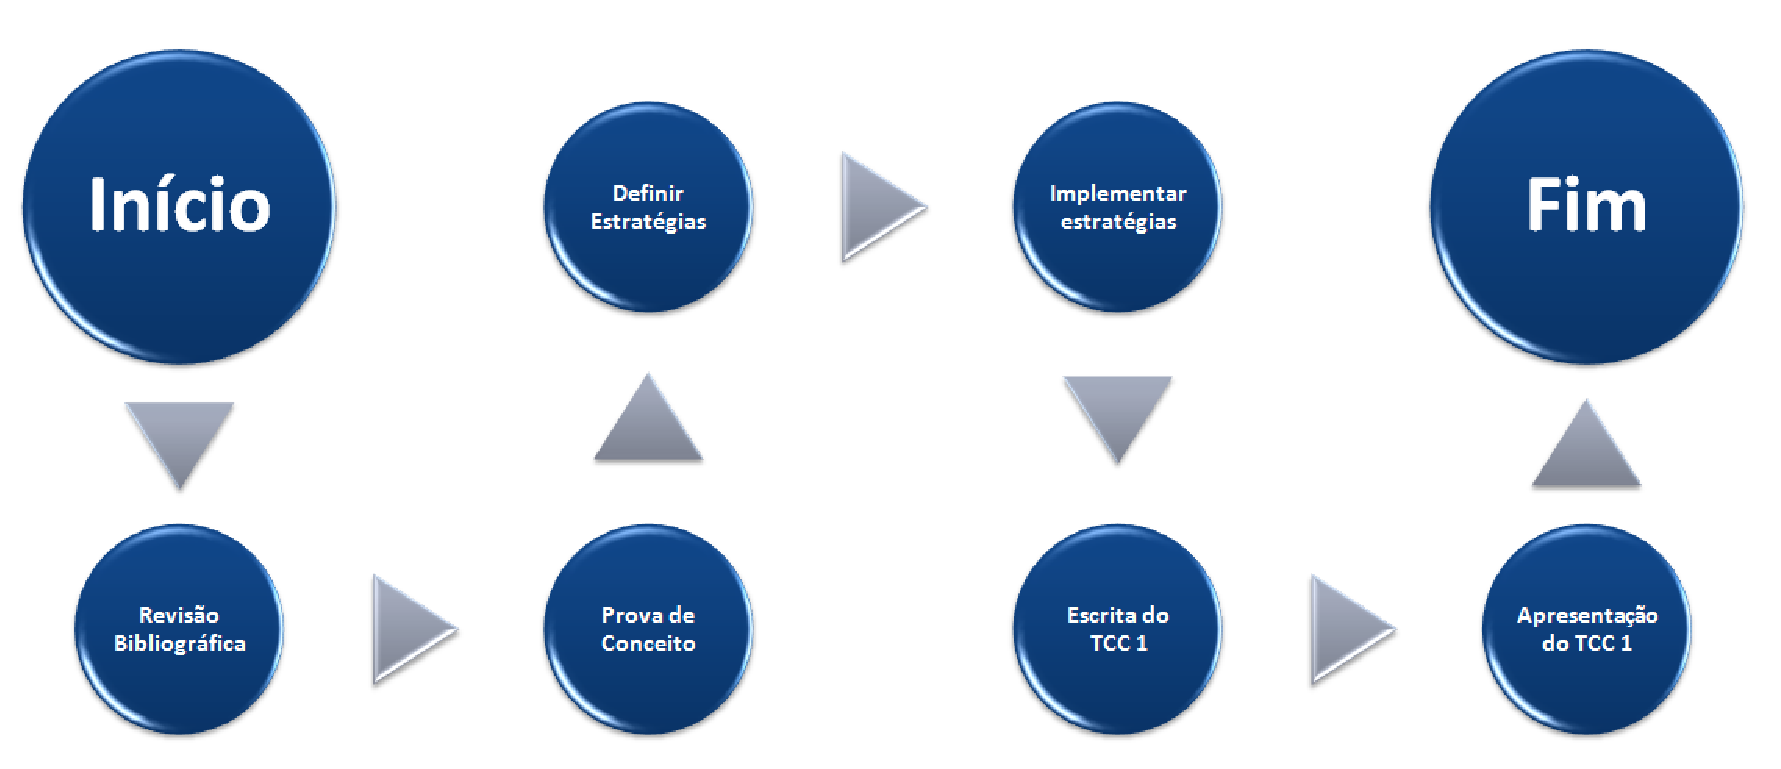
\includegraphics[scale=0.5]{figuras/metodologia.eps}
	\caption{Metodologia}
	\label{Metodologia}
\end{figure}

Primeiramente será realizada uma revisão bibliográfica, na qual serão levantados os principais algoritmos que serão executados sobre o grafo, bem como as principais práticas/padrões para o desenvolvimento de frameworks.

Após um estudo sobre o tema será realizado uma prova de conceito que definirá se o tema proposto é adequado ao período da disciplina. Em seguida serão selecionados os algoritmos mais adequados ao problema e uma proposta de arquitetura do framework será definida, além de definir quais serão as métricas a serem monitoradas durante o desenvolvimento.

Em seguida a serão implementados os algoritmos e a arquitetura do framework, considerando os intervalos aceitáveis das métricas definidas.

\section*{Cronograma}

\begin{tabular}{SSS} \toprule
    {Início} & {Fim} & {Fases} \\ \toprule
    {10/08/15} & {24/08/2015} & {Definir escopo} \\
    {25/08/15} & {10/09/2015} & {Estudo sobre grafos} \\
    {11/09/15} & {25/09/2015} & {Estudo sobre frameworks} \\ \midrule
    {26/09/15} & {30/09/2015} & {definir algoritmos a serem utilizados} \\
    {01/10/15} & {15/10/2015} & {definir arquitetura do framework} \\
    {16/10/15} & {21/10/2015} & {definir métricas} \\ \midrule
    {22/10/15} & {29/10/2015} & {implementar arquitetura} \\
    {30/10/15} & {05/11/2015} & {implementar algoritmos} \\ \midrule
    {06/11/15} & {27/11/2015} & {Escrita do TCC 1} \\
    {27/11/15} & {05/12/2015} & {Apresentação do TCC 1} \\ \bottomrule
\end{tabular}

\postextual

\bibliography{proposta} 

\end{document}
